%%%%%%%%%%%%%%%%%%%%%%%%%%%%%%%%%%%%%%%%%%%%%%%%%%%%%%%%%%%
% EPFL report package, main thesis file Goal: provide formatting for theses and
% project reports Template's Author: Mathias Payer <mathias.payer@epfl.ch>
% Thesis's Author : Arnaud Pannatier <arnaud.pannatier@epfl.ch>
%%%%%%%%%%%%%%%%%%%%%%%%%%%%%%%%%%%%%%%%%%%%%%%%%%%%%%%%%%%
\documentclass[a4paper,11pt,oneside]{report}
% Options: MScThesis, BScThesis, MScProject, BScProject
\usepackage[MScThesis]{EPFLreport} \usepackage{xspace}
\usepackage{array}

\title{A Control Plane in Time and Space for Locality-Preserving Blockchains}
\author{Arnaud Pannatier} \supervisor{Cristina Basescu} \adviser{Prof. Bryan
Ford}
%\coadviser{Second Adviser}
\expert{\color{red}The External Reviewer\color{black}}

\newcommand{\sysname}{FooSystem\xspace}

\begin{document}

\maketitle 

\maketoc

%%%%%%%%%%%%%%%%%%%%
\chapter{Introduction}
%%%%%%%%%%%%%%%%%%%%

%% Presentation and setting
Distributed ledgers are a becoming more and more used as they provide
independence to a central authority, anonymity, security of transaction,...
Some distributed ledgers as Bitcoin \cite{Bitcoin} managed to get a lot of
popularity for various reasons. However they still are subject to some
weakness. The purpose of this work is to advances the research concerning two
of them : World War III Scenarios and the time to validate a transaction.
Indeed, in Bitcoin \cite{bitcoin}, validating a transaction can take around one
hour, because it takes around ten minutes to validate a block, and it needs
around six blocks to be convinced with a high probability that the ledger won't
be forked, and the transaction invalidated. This might be okay for some
transaction of great value, for example if somebody is buying a car using
Bitcoin, this person might agree to wait one hour so that its transaction is
validated. However if somebody wants to buy its daily coffee using bitcoin, it
might be a bit annoyed with this waiting time. The other problem is World War
III scenarios. If a third World War occurs, splitting the world in two, one can
expect that the communication between the two sides might be cut. This is a
problem for regular distributed ledger as it will lead to forks that cannot be
resolved at the end of WW3.  This work is part of a bigger project called Nyle,
which uses the idea of locality to solve these problems. The idea is to
replicate the system along regions of different sizes, from local (e.g.
Switzerland, London) to global. With this idea a transaction can be validated
at a local region first, but it still possible to wait for global validation if
needed. Most of the time a transaction validated locally will be validated
globally as well, but in some case, when propagating the information to the
global regions, some transactions might be invalidated to avoid double
spending. For big transactions, people might prefer to wait for the global
confirmation. But if one wants to buy its daily coffee, local validation might
be enough for the merchant, especially if he saw the person every day. For
World War III Scenarios, Nyle offers a solution as well, indeed if a global
partition occurs, the system replicated in smaller regions that are not split
by a partition can still continue working flawlessly. 

%% Main Challenge
Nyle distributed ledger is maintained by nodes that are spread over the world.
Clients will then ask the nodes to proceed their transactions or other
requests. Nodes are participating to a different number of regions. A first
challenge is to draw these regions in a satisfactory manner. A second problem
is \textit{open-membership} : it should be possible for anybody with a
sufficient computational power and a good connection to maintain a node of the
system. This allows the system to be distributed. The challenge with
\textit{open-membership} is that nodes can join, leaves or move in the system
at anytime. This might not be a problem for classic distributed ledger as
Bitcoin \cite{Bitcoin}, as its protocol only take in account the computational
power that is in the system at a given time. But as Nyle is locality-based,
this might lead to additional challenges, each corresponding to the different
actions possible : joining, leaving and moving. For joining nodes, consider the
case where there was only a few nodes spread along a big region, for example
Western Europe, and after a while a large number of new nodes wants to join in
that part. If the region stays the same, this might lead to some problems,
indeed the consensus would take more time and the liveness could not be
guaranteed. Furthermore for a region of this size, the probability of a
partition is relatively important. One might want that in this case, additional
regions, corresponding for example to country might be created. This leads to
the idea that the regions should be able to adapt depending to node membership.
If nodes leave the system, this might lead to problems as well, indeed in the
inverse situation as before, some regions might not have a node inside anymore
that is maintaining the system. To avoid this situation, one might want to
adapt the region when nodes leaves to guarantee that a sufficient number of
nodes are in a region at any time. Moving nodes are creating problems as well,
if the region assignment is fixed but the nodes are moving, a node could be
after a while far away from the region it was assigned to. This might take a
while, but one can imagine the situation where a lot of nodes have moved far
away from their original position. In case of a global partition, this can lead
to the failure of even small regions, that is one problem that one wants to
avoid in Nyle. Therefore the regions should be adapted with the movement of the
nodes. 

%% Related work is insufficient

%% Description of the approach

%% Why it is needed.

%% Thesis Statement

%% Results 

%% Contribution

%%%%%%%%%%%%%%%%%%%%
\chapter{Related Work}
%%%%%%%%%%%%%%%%%%%%
This work builds upon several other works that are linked to the domains of
blockchains and locality. Nyle proposes a decentralized cryptocurrency using
different strategies than \cite{bitcoin-paper}, \cite{Dfinity}, \cite{Byzcoin},
\cite{Omniledger}, \cite{Monoxide} and \cite{Stellar}. It used them as an
inspiration source and share some aspects with theses general cryptocurrencies.
It is somehow orthogonal to them because it can use any of theses cryptocurrencies
as an underlying system and enhance them using the idea of locality to
add some partition-resistance to them. 

But some ideas are taken from these papers are used as well.  The
Sybil-resistance scheme used in the registration system is directly inspired
from \cite{Dfinity}, using \textit{endorsement} in the general way, which can
be in practice replaced by any Sybil-resistance scheme like Proof-of-Work
\cite{bitcoin-paper}. 

In particular this work tries to solve some drawbacks of traditional
cryptocurrencies like \cite{bitcoin-paper}, solving the problem of the waiting
time for validation by using region validation and making it resistant to WW3
scenarios. \cite{Byzcoin} and \cite{Omniledger} gives another interesting
solution to the waiting time for validation, but their results are orthogonal
to this research.

\cite{Omniledger} and \cite{Monoxide} uses sharding to increase performance.
Sharding splits the system in random committee that allow the fastest
processing of the transaction. This not directly related of what is done in
this work, as even if the system is split in different parts, it is not done
randomly but based on the locality, and the system is replicated in all the
regions. However, cryptocurrencies using shards can still be used as an
underlying system of Nyle, enhancing the performance of the partition-resistant
blockchain system created by this means.

This work is directly related to the locality-preserving algorithms developed
in \cite{CRUX} and compact-graph algorithms \cite{approximation oracle}. These
are described in detail in the next section. 

There is a class of algorithm that uses the idea of locality in a different
manner. For example \cite{Geo-DNS} or \cite{IP Anycast} use the idea of
locality to shorten the path for the packets, connecting the servers via the
closest path.

Replication is often used to guarantee integrity of the stored information
\cite{find-paper-replication}. In \cite{CRUX} and Nyle regional replication of
the system is used to create partition-resistance, and in Nyle it can be used
to allow region validation.

Classic consensus algorithms as \cite{Paxos}, \cite{PBFT} were used as an
inspiration to develop some parts of the theoretical algorithm. In practice,
and for efficiency, this work use \cite{BlsCoSi} that is much more efficient,
using trees for communication.  

This works uses a distributed public algorithm for the source of randomness
like \cite{RandHound}. Each node will use this source to draw a random level.
The way it is used is described in detail in the next section. 

%TODO : Add Stellar

%%%%%%%%%%%%%%%%%%%%
\chapter{Background}
%%%%%%%%%%%%%%%%%%%%

%%%% Plan
% - Crux (??)
% - Nyle (7-8p) - General description - What is already implemented - Next
%   steps
% (motivation for the control plane)
%%%%%%%%%%%%%%%%%%

This Master Thesis is part of a biggest project that concerns
locality-preserving systems. In particular, it builds upon
CRUX\cite{basescu2014crux} and is part of Nyle.This section describes the two
different projects. 

\section{CRUX}

%%%% General Presentation
% - Solution to partition
% - General idea
% - Small Overhead
% - Generality 
% - CAP Theorem
%%%%%%%%%%%%%%%%%%
\subsection{General Presentation} CRUX introduces a smart way of dealing with
partitions in decentralized systems. The purpose is the following : partitions
occur in decentralized system. But one can maybe try to find a solution to
reduce their effects on the global system. For example, if a partition occurs,
there is no reason that nodes that are functioning in the same side of the
partition should stop working because of the partition. 

The general idea is that a system can be replicated at different scales, from
local (cities, region) to global.  With the additional property than each
replicated system will continue to work correctly if no partition splits it. If
a global partition occur, then the global region might not work, but all the
replicated system in local regions will still continue working. This is a
direct solution to the previously mentioned problem : nodes working on the same
of the partition will continue to work.

Obviously, this solution comes with an overhead, as the system should be
replicated in all the regions. But there are some ways of reducing this
overhead, in a way that it stays reasonable and that the resistance to
partition is maintained. To reduce this overhead, CRUX algorithm for regions
creation presented below ensure that the proper number of regions is created,
in a manner that the number of regions created induce a reasonable overhead and
that the partition resistance stays efficient. If CRUX is used for a
particular, known system, overhead can be even more reduced.  As the systems
are replicated in every region, most of the data is replicated along the
regions. So one might actually dig inside the specification of one system and
manages not to store twice the same data. But this overpass a bit the goal of
CRUX, which wants to be the more general possible. 

Indeed, the force of CRUX is that it is applicable to any distributed system,
as no particular hypothesis on the system is made. It only starts from one
simple idea : one system can be replicated at smaller scale to ensure partition
resistance. 

% TODO : do more research on that.
A note should be made about the CAP-theorem. Recall that this theorem states
that no system can be consistent, available and partition-resistant at the same
time. It seems that this solution is adding partition tolerance to available
and consistent system. Thus leading to the violation of the theorem. But it is
not exactly the case, as the enhanced system only ensure that nodes can still
work in the same side of a partition. The regions split by a partition are
not working anymore. Even if the system can still work on the same side of a
partition, it's not totally partition resistant.

%%%% Common Tools
% - Approximation distance oracle
% - Bunch
% - Cluster
% - ARA 
%%%%%%%%%%%%%%%%%%
\subsection{Common Tools :  ARAs} 
This section describes how to create the regions that are used to replicate the
system. These regions are used by Nyle as well, therefore we will describe it
in detail. These regions are called \textit{Available Responsive Areas}, in
each region a copy of the replicated system is deployed. To create these
regions each node will participate first at a lottery. Each node starts at
level 0. Then each node go to the next level with a given probability $p$. This
procedure is repeated at each level, and is stopped when no nodes are promoted
to the next level. This first empty level is called $k$. Then each node can
compute two quantities that will be necessary to create \textit{ARAs} : their
bunch and their cluster. 

\begin{table}[] 
\centering
\begin{tabular}{rrrrr}
Levels/Nb of Nodes & 100 & 200 & 500 & 1000 \\ \hline
\multicolumn{1}{r|}{0} & 90  & 180 & 450 & 900  \\
\multicolumn{1}{r|}{1} & 9 & 18  & 45  & 90   \\
\multicolumn{1}{r|}{2} & 1   & 2   & 5   & 9 \\
\multicolumn{1}{r|}{3} & 0   & 0   & 0   & 1  
\end{tabular}
\caption{Example of lottery with $P = 0.1$ where $k= 3$ for $N= 100,200,500$
    and $4$ for $N = 1000$}
 \end{table}

\paragraph{Bunch} A node can compute its bunch in the following manner. It
looks at every other nodes by order of distances in ascending order and
includes it in its bunch if its level is not smaller than the one it encounters
so far, including its own level. 
% TODO include image of Bunch

\paragraph{Cluster} A cluster is a complementary concept. The cluster of node
$A$ is defined as the set of other nodes that have $A$ in their bunch. 
% TODO include image of Cluster.

The smallest region radius $R_{min}$ is defined for the whole system. Each node
will construct ARA's around itself starting at $R_{min}$ and doubling the
radius at each time. It stops at the first ARA's that is covering its entire
cluster. 

By the lottery, most nodes will be level-zero nodes. Therefore their cluster
supposed to be small, conducting to the creation of a small number of ARA's.
The small number of nodes that are at level $k-1$ will have every other nodes
in their cluster by construction. This means that there will be at least one
ARA that covers the whole system. 

%%%% Nyle
%  - Problems it solves - Link with CRUX - Environment - Type of Blockchain 
% - What is already implemented 
% - Next steps. 
%%%%%%%%%%%%%%%%%%%%%%%%%%%%%
\section{Nyle}

Nyle is cryptocurrency that uses locality to answer some classical problems of
a blockchain systems. Two main problems are addressed: WW3 scenarios and
approval time for a transaction.
 
\paragraph{WW3 Scenarios} \label{WW3} In case of a WW3, we can expect to have
at least a long-lasting partition that will split the system in two. This is a
problem for classical cryptocurrencies like \cite{bitcoin-paper}, because for a
block to be approved, the users are supposed to wait to have a global
consensus. This consensus will not be reached with a long-lasting partition and
therefore it will create problems for classical cryptocurrencies. Nyle solve
this issue by design using locality.

\paragraph{Approval Time for a Transaction} \label{approve_time} Another issue
with waiting global consensus is that it usually takes a long time. If a
customer wants to use a cryptocurrency in a daily life, the nodes should be 
able to validate (at least partially) a transaction relatively fast. The
solution provided by Nyle use locality again: with Nyle a transaction is
validated at different levels, and it is up to the customer to wait a local, or
global validation for a transaction. For small transaction, for example for
buying a coffee, the customer might agree to only have local validation. For
bigger transaction he might wants to wait a bit longer to have global
validation.

\subsection{Locality : From CRUX to Nyle} Nyle uses ARA as the representation
of one region. In each of these regions there will be a copy of the same
system, in the case of Nyle the system is a blockchain. So each region will
have its own blockchain and validate all the transactions between the nodes
that are included in it. Some nodes can be included in different regions, and
they will send their transactions to all the regions they are part of. Which
ensure that each blockchain will be updated each time there is a transaction
that concerns one of its nodes.

\subsection{Stable Environment vs Byzantine Evolving System}

The big difference between CRUX and Nyle is that the purpose of CRUX is to work
in environments where machines are relatively "stable" which means that they
are not supposed to churn or to crash often, and more, where the machines are
not supposed to move. This is not the case for Nyle : if we have a
cryptocurrency, we can expect to have malicious, deficient and/or moving nodes.
This will add some difficulties that will be managed by the protocol.

\subsection{Blockchain System} \label{blockchain_subsection}

Each region will have its own blockchain, in Nyle the choice for the blockchain
will be chosen between Omniledger or ByzCoin. But it can be generalized to any
kind of blockchain.

\subsection{What is already implemented for Nyle} \subsubsection{Transaction
validation} We already have a protocol that validates a transaction.

\subsubsection{Block storage on node} As each node will participate in
different regions (from very local to world-wide), it will need to store the
blockchain for all of these regions. We have a method that reduces the
redundancy, by only storing the hash of a block instead of the full block at
each level. 

\subsubsection{Proof-of-Location} We already have a protocol for controlling
the distance from a new node to the rest of the nodes. And that assures no one
cheats by giving false distances. 

\subsection{Next Steps} Here is the structure of Nyle :

\begin{itemize} 
\item Based on the proof-of-location, build a CRUX-like network
\item In each of the region of the regions build a Blockchain 
(see \ref{blockchain_subsection})
\item Use the transaction validation to  give info on the validated region
(see \ref{approve_time} (Approval time for a transaction))
\item Dealing with moving actors.
\item Dealing with double-spending issues
(if a node spend the same coin in different regions) 
(see \ref{WW3} WW3 Scenarios) 
\item (Investigate if this design is open to other errors)
\end{itemize}

%%%%% TODO : add general description 
%%%%% Motivation
% - Already have a system working for non-byzantine no-churn system 
% - Dealing with these problems can be done by dealing nodes insertion,
            %   deletion and moving.
% - If we solve that then we can return to the previous system and everything
            %   should be working
%%%%%%%%%%%%%%%
\subsection{Purpose of this project : motivation for a control plane}

CRUX proposes a system that is working in a stable system (with low-churn) and
where nodes do not move too much. As this situation corresponds to some
systems like wide-area database, ... It is definitely not the case of a
cryptocurrency.  For these kind of system, one can expect to have at least some
churn, some moving nodes and some adversarial nodes.  If the system has a
precise protocol for dealing with nodes entering, leaving and moving in the
system, then the problem of the evolution of the system is solved. Indeed the
churn phenomenon can be described as some nodes leaving the system and
optionally reentering later. 

Therefore the purpose of the control plane will be to deal with the evolution
of the regions that follows the evolution of the nodes in the system. Once that
problem is solved, the blockchain can be replicated in the evolving region and
the strategy will be the same as in CRUX. 

Thus this project introduce a control plane, that is in charge of the evolution
of the nodes in the system. In particular, it will be in charge of dealing with
the nodes joining, leaving and moving in the global system. If the blockchains
is replicated in all the regions, the control plane will be global. 

%%%%%%%%%%%%%%%%
\chapter{Control Plane : Design}
%%%%%%%%%%%%%%%%

%%%%%%%%% 
%  - Problem definition (Hypothesis, Goals, ...) (2-3p) 
%%  - Hypothesis on the threat model
%  - First version: Simple Control Plane (15-20p ?) 
%%  - Graphs: Control flow, Protocol flow trough time 
%%  - Tools: Description of each subprotocols 
% %%%(consensus via Blscosi, gossips protocols, ...). 
%%   - Discussion
%%%%  - Advantages, prove that it fulfils the goal
%%%%%%  - Graph of difference between system without control plane and with. 
%%%%  - Drawback (evaluation of computational, memory and communication costs)
%%%%%%  - With graphs
%%  - Security  Analysis 
%%%%% - 2-3 scenarios illustrating malicious behaviors (written and/or with implementation)
%%%%%%%%%%%%%%%%%%%%%%%%%%%%%%%%%%%%%%%%%%%%%%%
This part will describe the design of the Control Plane, which has the mission
to solve the problem of node insertion, deletion and movement inside the
system. Allowing to use a CRUX-like region creation algorithm in an environment
with churn. 

\section{Problem definition}
%%%%%%%%%%%%%% Problem definition
%% Hypothesis : 
%%   - one-to-one communication
%%   - synchrone network
%%   - Correlation between pings and distances
%%   - Nodes are malicious
%%   - Adversary can delay communication
%%%%%%%%%%%%%%%%%%%%%%%%

\subsection{Hypothesis} Three hypotheses are made on the network. First it
assumes an internet-like network with one-to-one communication. Each node is
able to contact any other nodes. The network is supposed to be synchrone. This
means that every message sent by a node to another will arrive in order, and
that a message that is sent will be received within a given window of time. The
third hypothesis is made on the geometry of the network. It states that for
small pings (under 100ms) the ping time is actually correlated with the
distance between two nodes. This is a result from \cite{locality-result} on
which we build the locality properties of the system. 

\subsection{Threat model}
%% Todo : when adversarial model is done, depending on results. 

%%%% mostly copied from
% https://docs.google.com/document/d/1xz1jTphKqxxkAucdh_oOqsFXH147Cjlzcnjmt-yx-f8/edit#heading=h.aq4k1vxbt0t0
\section{General Presentation}

The Control Plane is composed of five different components [FIG.
\ref{fig:modules}], each necessary to solves different part of the problem. It
needs a membership component, to define precisely which nodes are in the system
at any time. It needs a locality component which gives the distance between two
nodes in the system. Then it needs a region management component, which will
draw the regions based on the membership and the locality. The time will be
split into epochs, a component is in charge of dealing that aspect. And
finally, the control plane is in charge of answering some requests linked to
the location and presence of the nodes in the system. Each will be described in
detail below. 

\begin{figure}[!h] \centering
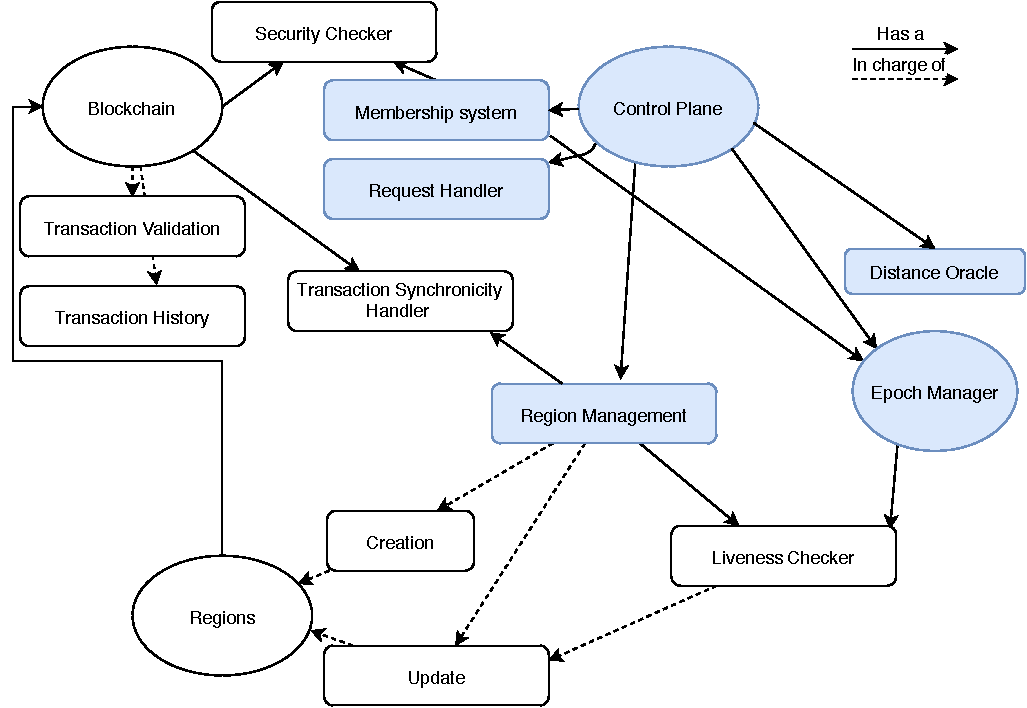
\includegraphics[width=400pt]{figures/Nyle_components} \caption{List of modules
of Nyle} \label{fig:modules} \end{figure}

\subsection{Membership Component}

At each epoch, a registry contract containing a summary of all participants is
created. Registration use endorsement (for example solution to a proof-of-work
problem).  This system will be global. Nodes can ask the participants of the
system to know the identity of other nodes. To validate a new contract  it
should be signed by the majority of the nodes of the previous epochs.

\subsection{Locality Component}

 The role of the locality component is to give all pairwise latencies between
 nodes of the system. We assume it already exists (distance oracle), or it can
 be computed by nodes. In the first model all pairwise latencies is computed
 between each node and every node agree on them via consensus. 
 
 \subsection{Region Component} This component is used to create and update
 regions. For the simple case, this part will be based on CRUX. At each epoch
 CRUX is run based on the new registration, and regions are created.
 
 \subsection{Epoch Component} The epoch manager is linked to the membership
 system (we allow to change membership at the beginning of one epoch). New
 nodes can join at the beginning of one epoch. If nodes have moved, the region
 component will change or maintain their assignment at the beginning of one
 epoch. 

Epochs happen at a defined rhythm (e.g. one day). This frequency can be
shortened to ensure that nodes that want to join do not wait too long, or made
longer if one wants regions not to be redrawn too frequently. 

\subsection{Request Handler} The control plane is the right part to get
requests as it is aware of the nodes location and region assignment. It will be
in charge of answering the request for nodes assignment and nodes location. 

\begin{figure}[!h] \centering
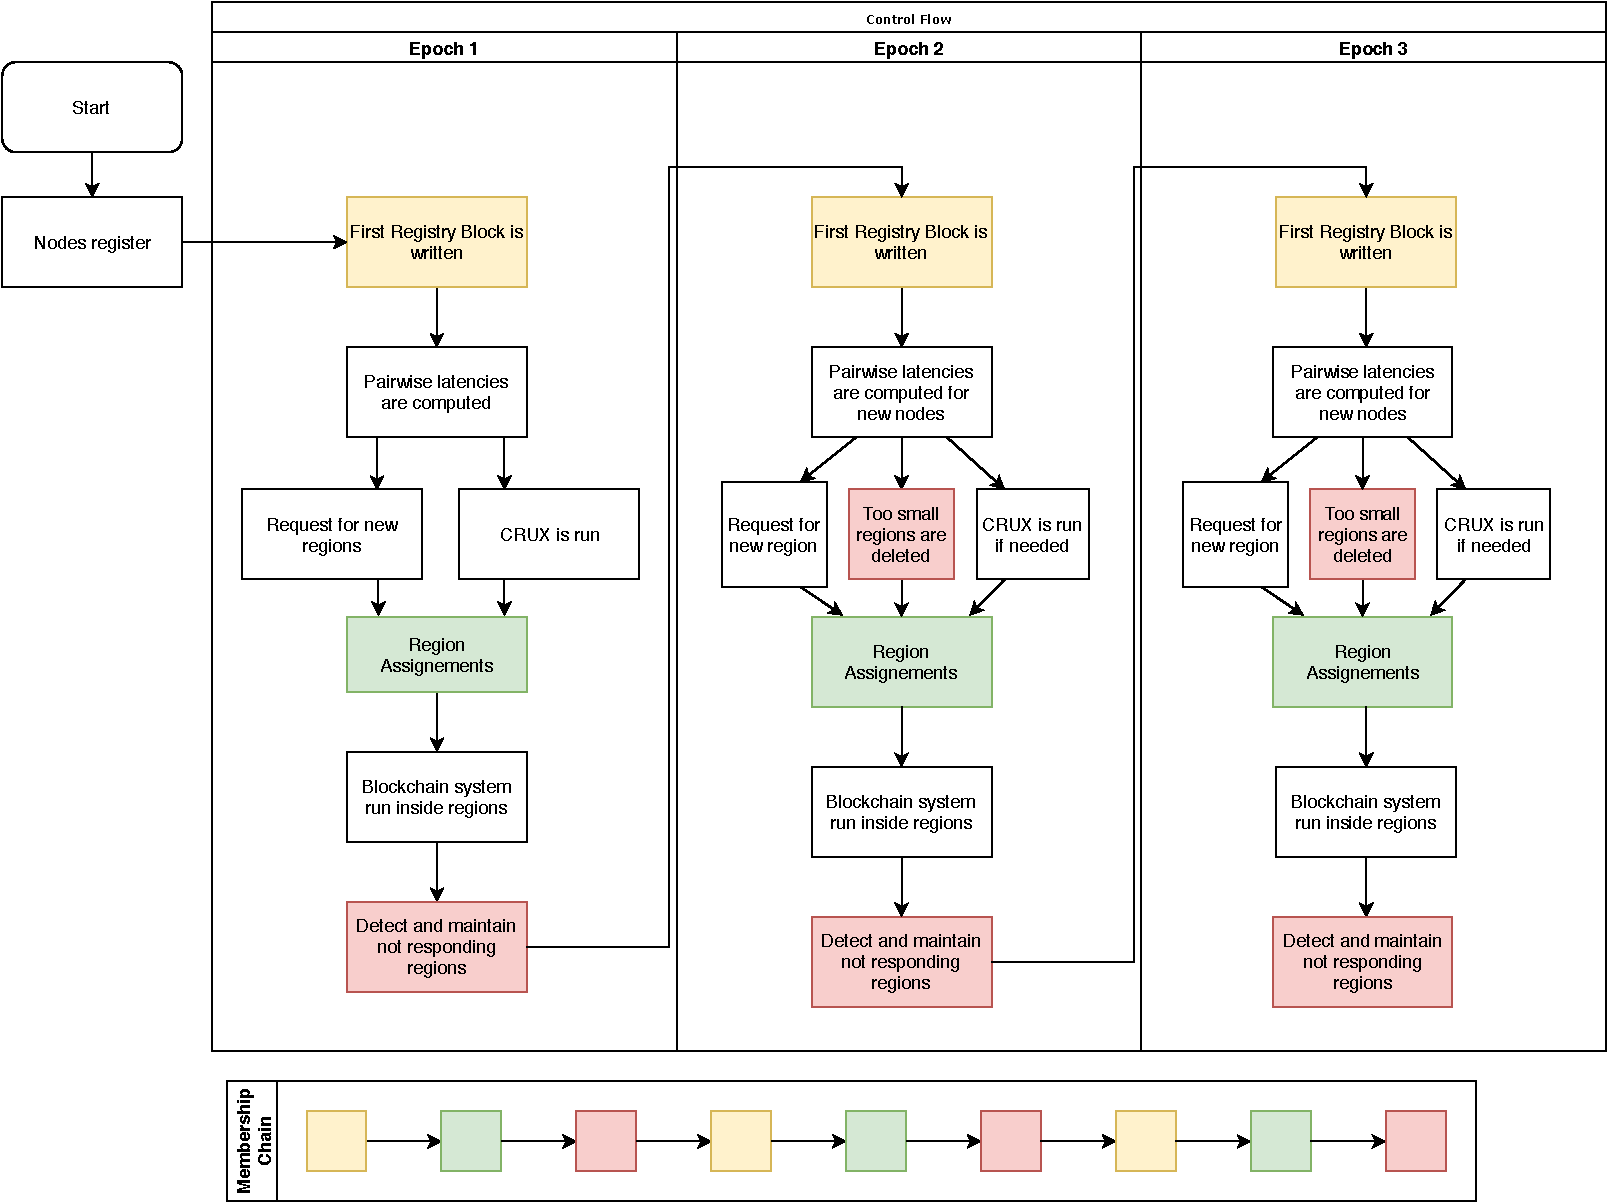
\includegraphics[width=400pt]{figures/Nyle_controlflow} \caption{General control Flow
of Nyle} \label{fig:controlflow} \end{figure}

\section{First version : Simple Control plane} This version presents the first
version of the Control Plane. In which most of the work is done on the
membership component. At each epoch nodes can join if they manage to get an
approval from the member of the previous region. The locality component in this
model is brute force : every node computes its pings to every other nodes and
consensus is made on that information. The region component in this model is
really simple : based on the registration, and the pings, CRUX is run at each
epoch. Redrawing the map of the entire system. 

\subsection{Membership Protocol}
This section describes the membership protocol [FIG. \ref{fig:registrationprotocol}].

\begin{figure}[!h] 
\centering
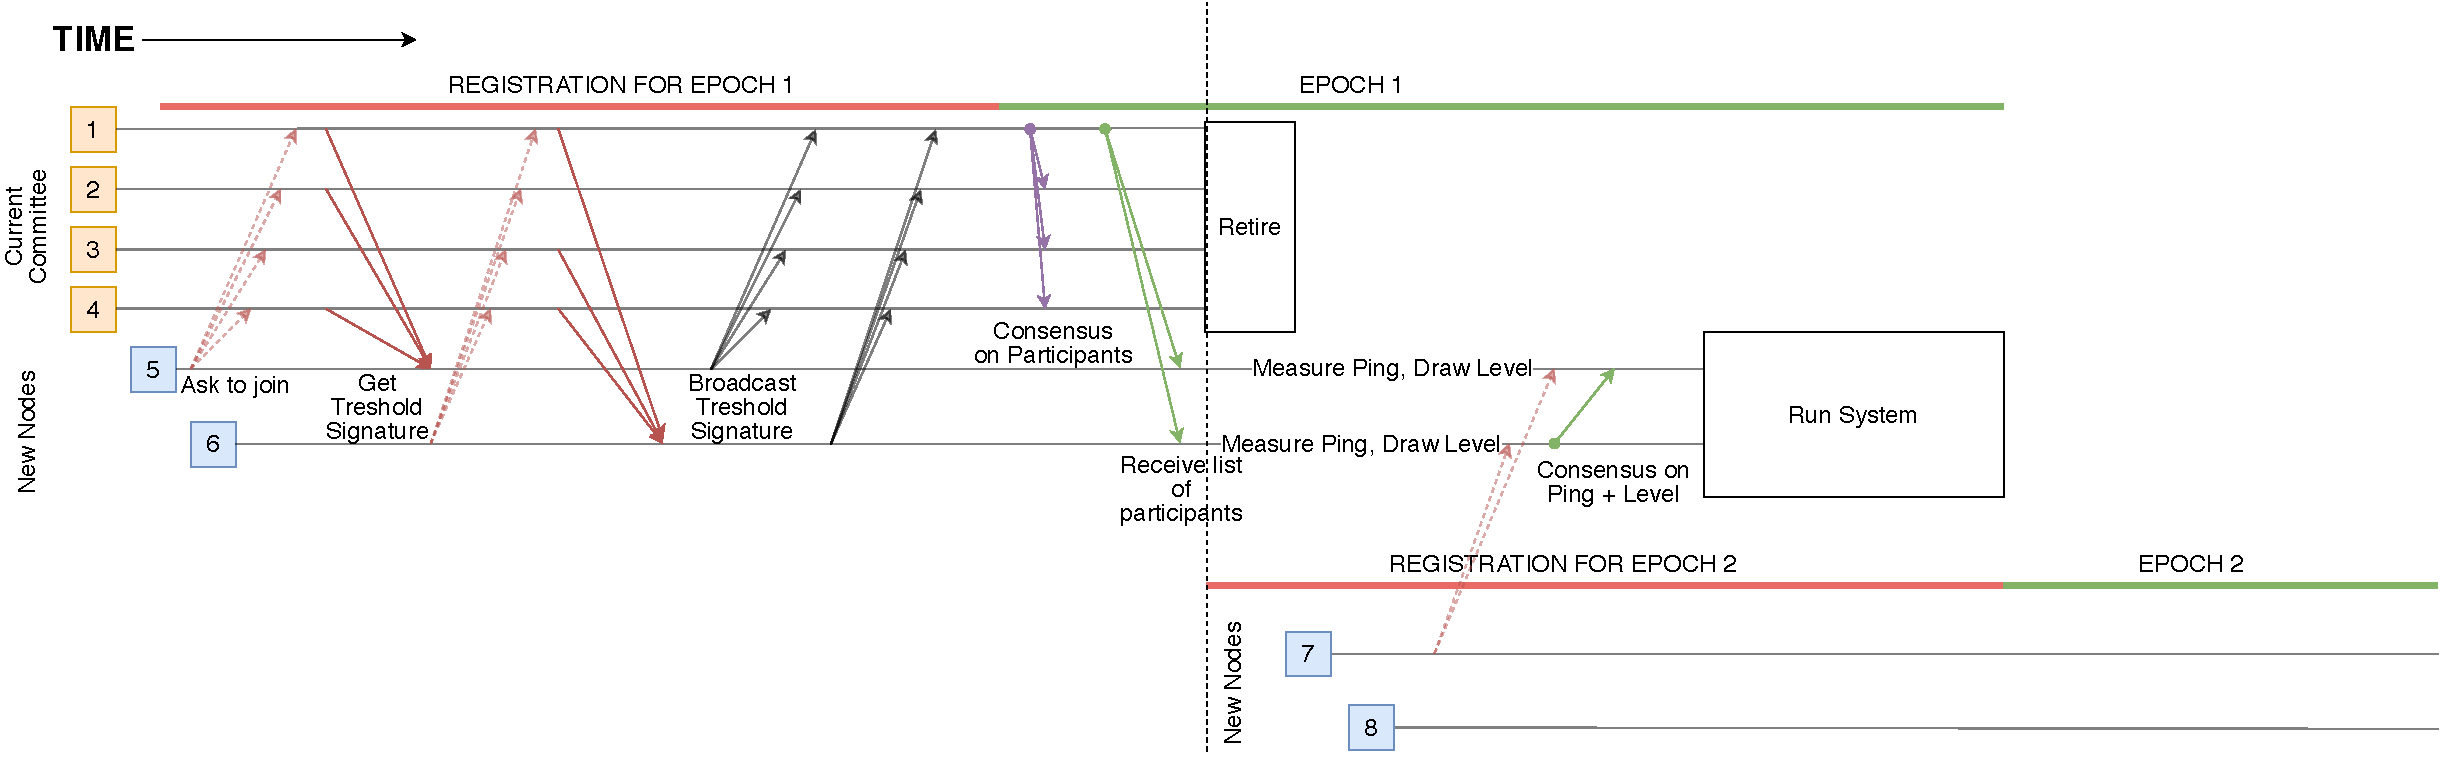
\includegraphics[width=400pt]{figures/Registrationprotocol}
\caption{Sketch of the Protocol}
\label{fig:registrationprotocol}
\end{figure}

The system will go through some cycles (called epoch) of two different phases :
the registration period and the live period. The first period is actually there
to manage the participants of one current epoch, and the “underlying system”
(for example a cruxified-blockchain) will be run during the live period. Assume
that each node has a synchronized wall-clock which gives the time of the
different periods.

The authority that will decide which node participates in the next epochs are
the participants of the current epoch, which will be called the admission
committee. Assume that a set of genesis participants, which will be the first
admission committee, exists.

\paragraph{Registration Period}
If a node wants to register for the next epoch, it has to send the following
information to the admission committee : a name, a public key, and an
endorsement (for example solution to a proof-of-work problem) and ask for a
threshold-signature. 

If the new node manages to get back a threshold-signature from the current
committee, it has to broadcast it again to the admission committee during the
same registration period. The current committee will then acknowledge that it
is a participant for the next epoch. The admission committee will aggregate the
threshold-signatures for all the participants for the next epoch. At the end of
the registration period, the admission committee will reach a consensus on the
new participants, by threshold-signing the list of the members.  

\paragraph{Live Period}
At the beginning of the live period, one member of the admission committee will
send the threshold-signed list of the participants to the current members. If
one of the participants did not receive the list, it can ask any member of the
admission committee to have it. After that propagation, the admission committee
can retire, and the member of the current epoch becomes the new admission
committee. Then members of the new epoch will compute ping-distances between
each other. Participants will as well draw a level from unpredictable,
bias-resistant public randomness source. They will then reach consensus on
those ping-distances and levels by threshold-signing them and rebroadcast them.
At this point each member of the new epoch will have the same view of the
system (participants + pings + levels). Therefore these participants will be
capable of running the system in a deterministic manner.

Following the election of the new admission committee at the beginning of the
live-epoch, the registration period for the next epoch can begin, as the
authority that will accept admission is running. Registration period and live
period can therefore be superposed [FIG. \ref{fig:registrationprotocol}], which
permits to have a system running at every time. 

\subsection{Threshold-Signing Admission}
To get an admission a node that wants to join for the next system will use the
BlsCoSi protocol \cite{BlsCoSi_protocol}. it will generate a tree with him as
the root and the admission committee as nodes in the tree. Each node of the
admission committee will have the choice of signing or rejecting the admission
query. The threshold will be set at the majority. So if a node manages to get a
majority of signatures then it will be accepted in the system, A node from the
admission committee is supposed to accept the query if it has not already seen
the node, and if the endorsement is convincing and was made with the public-key
associated. This ensures that a node cannot steal the endorsement of another
for registration.  

%%%%%%% Committee consensus
\subsection{Committee Consensus}
Committee consensus is used at two different times. First at the end of the
registration period. Consensus should be reached by the admission committee to
the participants of the next epochs. A random member of the admission committee
is selected to run the consensus protocol. It will send the list of members
that it aggregated during the registration period. And try to get a threshold
signature on it from the other member of the admission committee. Members of
the admission committee are supposed to sign the list if they aggregated the
same list of members for the next epoch.

If one member does not manage to reach consensus, another can be selected to
run the consensus. A communication round can be added between two consensus
phases in order that every member of the admission committee broadcast its list
of members with valid proofs.

The same idea is used at the beginning of the live epoch to reach consensus on
the list of pings between every member of the system and on the levels on all
nodes in the system.
% TODO : think on what to do if the consensus is not manageable. 

\subsection{Public distributed source of randomness}
To draw the level to run the region creation algorithm, a distributed public
source of randomness will be used. This can be targeted by adversaries trying to
get a higher level and thus a higher place in the system. To be sure that this
source is not targeted, it is  based on the information created during the
consensus on the participants just before drawing the regions. 

\section{Discussion}
\subsection{Advantages}
This simple version of the control plane is actually solving the problem of
churn and nodes movement in the system. A comparison will be made with a fixed
version only using CRUX for region management but without control plane. The
system begins with a fixed number of nodes and create regions based on CRUX,
then the system is replicated inside all regions. 

\subsubsection{Nodes insertion}
The version without control plane cannot add nodes to the system. Indeed a
fixed number of nodes is required to create the regions. With this control
plane, node insertion is possible at the beginning of every epoch.
% TODO add image

\subsubsection{Churn resistance}
Nodes can churn. If the system is not supposed to change, crashing nodes can be
still in the system. With this control plane, nodes that have crashed cannot
register for the next epoch and therefore are removed from the system. 
% TODO add image 

\subsubsection{Adaptation to Node Movements}
Nodes can move as well, if the regions are only drawn at the beginning of the
system. Then it's possible that after a while a lot of nodes have migrated from
where they were at the time that the regions were drawn. This might be a
problem, indeed, the purpose of the replication was to ensure that in case of a
partition, nodes participating in the same side of the partition should still
be able to work. If most of the nodes have moved, but are still participating
in the region of their first assignment, a partition could happen somewhere in
the system leading to failing regions that should be on the same side of the
partition. The control plane solves this problem as the region are redrawn at
each epoch taking account of the movement of the nodes. Increasing the
partition resistance, with the movement of nodes.
% TODO add image

\subsection{Drawbacks}
This control plane is simple and reach its objective, but it requires a lot of
resources. Some of the drawbacks of this approach are listed below. 
These drawbacks are addressed in the section Improvements.  

\subsubsection{Control Plane is global}
If the system is replicated in all the regions, the control plane itself is
global. Meaning it could be subject to a partition. In this case the replicated
system would continue to work, but the control plane could only continue to
work on the side of the majority. This is not a major drawback as the main
purpose, the continuity of the subordinate system is guaranteed.

\subsubsection{Epoch Transition Requires Resources}
Epoch transition requires a lot of resources, indeed first it needs a lot
communication for the consensus and the registration as every node that were
previously on the system should be contacted by every new node. If $N_i$ is
the number of participants at epoch $i$. Then registration for epoch $i+1$
requires $O(N_i * N_{i+1})$ messages. As every new node has to send a message
to every member of the previous committee. This can be really inefficient. 

Then when the registration is done, the protocol as it is will redraw most of
the regions as the algorithm for region creation is reused. This can be
inefficient as well, and it is then for the transition to happen, a copy of the
whole underlying system at epoch $i$ should be replicated in each new region of
epoch $i+1$.

%% TODO FIT
\begin{figure}[!h] 
\centering
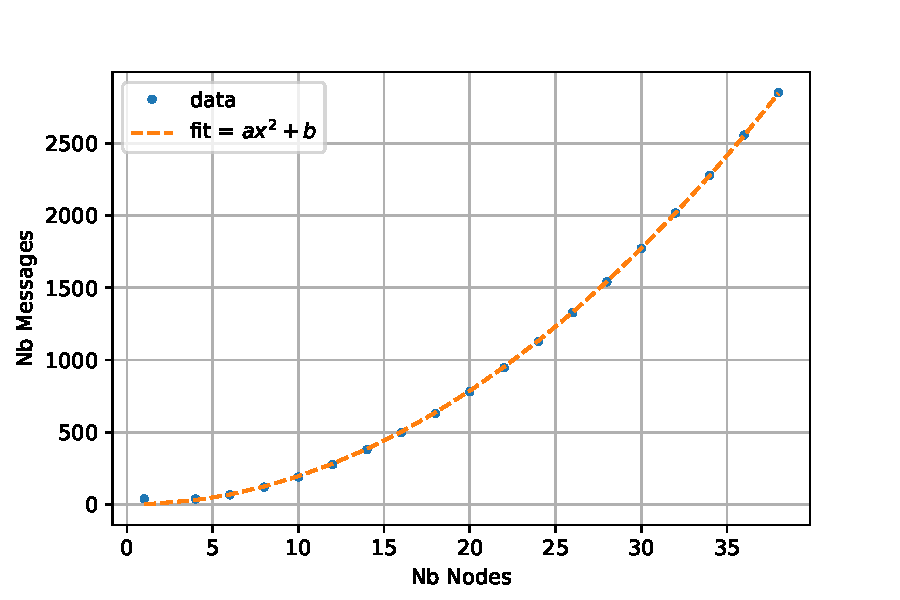
\includegraphics[width=350pt]{figures/messages-plot}
\caption{Growth of the number of messages for one epoch with the number of nodes.}
\label{fig:messages-plot}
\end{figure}

%% TODO FIT
\begin{figure}[!h] 
\centering
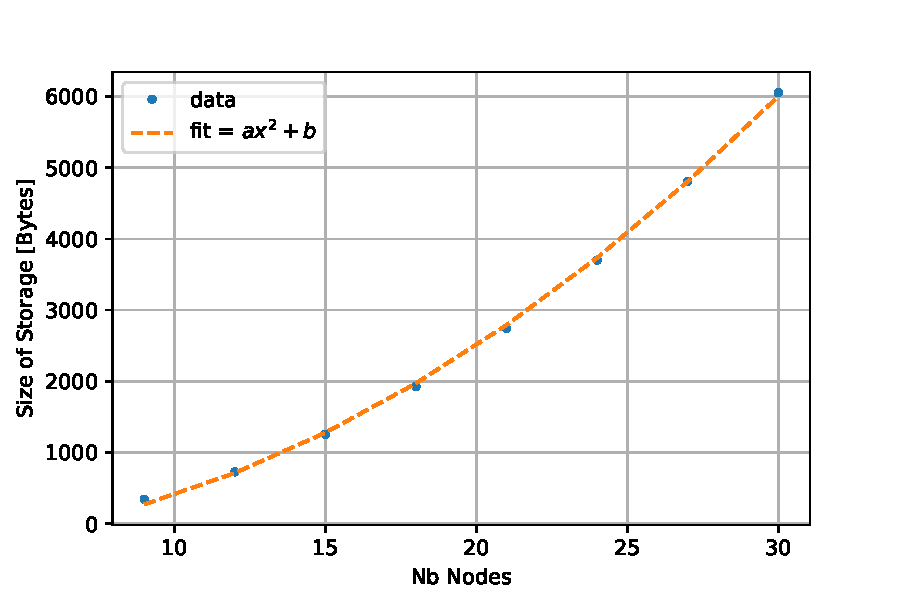
\includegraphics[width=350pt]{figures/storage-plot}
\caption{Growth of the number of storage for ping distances for one epoch with
    respect to the number of nodes.} \label{fig:storage-plot}
\end{figure}

 
\subsubsection{Omniscience of the Nodes}
Nodes are actually aware of a lot of information. By design they are aware of
the list of every other nodes in the system, their levels, the pings between
each pair of nodes in the system, all the region created and all the region
assignment. The nodes need to be aware of this information in order that
every node will run the algorithm for region creation and arrives to the same
regions. But this can be a lot of information to store.

\section{Security Analysis}

\subsection{Threat Model}
Attacks on the system can be made internally (from malicious nodes) or
externally by delaying the interaction between nodes or intercepting and
changing messages. We will give the precise portion of malicious nodes that
this protocol can handle. In this threat model, malicious nodes are regular
nodes that decides to act against the system. In particular, malicious nodes
have only access to a bounded computational power, and they cannot break the
cryptographic primitives. 

\subsection{Network Attacks} 
\subsubsection{Man-in-the-middle attacks} \label{MitM}
The messages exchanged during the protocol are the following: 

\begin{table}[]
\begin{tabular}{p{0.05\textwidth}p{0.3\textwidth}*{2}{>{\arraybackslash}p{0.2\textwidth}}}
& Message                                                                                                       & Signature                                                       & Effects of a Sufficient Delay \\ \hline
1 & Join request                                                                                               & Requesting node                                           & Request refused               \\
2 &Threshold signature of the request                                                             & Threshold number of the current committee & Request refused               \\
3 &Broadcasting of the Threshold signature                                                    & Threshold number of the current committee & Request refused               \\
4 &Messages for the consensus on the participants,
list of the participants                                                                                       & Leader of the current committee                   & View Change                   \\
5 &List of pings and levels                                                                               & Leader of the current committee                   & View Change                  
\end{tabular}
\caption{List of the messages exchanged during the protocol. The signature of the message and the effects of a delay are given. }
\label{tab:my-table}
\end{table}

As all the messages are signed, if a message is changed, it will be noticed by
the receiver. Which will discard the altered message, and ask again to the
sender.  Therefore the only effect of a Man-in-the-middle attack will be to
delete some of the messages, which is a sort of delay attacks. 

\subsubsection{Delay attacks}
This protocol is not really resistant against delay attacks. It assumes
wall-clock synchronicity between the nodes, which can cause some problems. The
effect of a delay of message are listed in [TAB. \ref{tab:my-table}]. During
the registration, if the messages are delayed until the start of the next
epoch, then it will lead to the refusal of the request, and the node have to
create a request again for the next epoch. If the messages of the leader of the
consensus for the participants of the pings and levels are deleted or delayed,
the other nodes will ask for a view change : asking the next node in the list
to start the consensus. 

\subsection{Malicious Nodes}
\subsubsection{Consensus}
If a malicious node is already in the committee, the only misbehavior that it
can do the period is to refuse to sign the message. Re-sending wrong messages
are already treated in \ref{MitM} and it's not possible to forge them because
of the signature. Refusing to sign join requests can lead to a failing protocol
if the number of malicious nodes is bigger than the threshold required to get
the signature. As the signature procedure is done using BlsCoSi \cite{BlsCoSi},
the registration process is subject to the same threat. BlsCosi is an efficient
way to implement The \textit{Practical Byzantine Fault Tolerance} (PBFT)
algorithm which guarantee \textit{safety} and \textit{liveness} if the system
as no more than $f$ faults among $3f+1$ malicious nodes.Therefore it is
required to have no more than $f$ malicious nodes, where $f$ is given by : $3f
+ 1 = N$, where $N$ is the number of nodes in the current committee. As the
number of nodes in the system evolves with time, it required not to have more
than this fraction of malicious nodes in the system at any epoch. If for one
epoch, the number of malicious nodes is bigger, then they can block all the
consensus, leading to a failing system. 

If a malicious node is elected as a leader of the consensus on the list of
participants or on the nodes, it can decide not to start the consensus. After a
while, another node will be elected to run the consensus, which will eventually
succeed if the number of malicious nodes is low enough.

\subsubsection{Attack on levels}
At the beginning of one epoch, nodes compute their bunch and cluster based on
the pings and the level that is drawn from a shared public source of randomness
which is renewed at each epoch. Nodes deploy region covering its cluster. Each
node will participates in regions along its bunch. This procedure however is
not based on the action of a nodes, but just on the fact that they exist at a
given place and a given level. What is meant by that is that every nodes have
the same view of the system. And if node $A$ have node $B$ in its bunch, then
node $A$ is supposed to participates in a region which is based on the position
of $B$ and spans the cluster of $B$, but $A$ already has all the informations
to know about this region using only the pings and levels. Therefore node $B$
cannot use a high level to perform action that will block the system. 

However, if a malicious attacker could take over the lottery process, it could
manages to group the high level in a side of the system. Leaving only the
level-zero. This could lead to some problem [App \ref{Problem with
levels-zero}]. Taking over the lottery process should'nt be possible by design.
Indeed, the lottery is based on a public source of randomness that renewed at
each epoch, and revealed after the registration of the levels. 

Nodes can know the level of other nodes, because they base the compute of their
levels on the threshold-signed list they received from the previous committee.
It is important that the source is revealed after registration of the levels,
otherwise malicious nodes could try to influence the order of the list on which
the lottery process is based. 



%%%%%%%%%%%%%%%%%%%%
\chapter{Improvements}
%%%%%%%%%%%%%%%%%%%%
This section proposes some improvements to the simple control plane approach. They
are supposed to address the drawbacks of this simple protocol, each improvement
will be illustrated in a Strawman model. Finally, an advanced
version of the control plane that uses a region creation algorithm based on
time/space graphs will be proposed. 

\section{Strawman 1 : Locarno Treaties} \label{Locarno}

\begin{figure}[!h] 
\centering
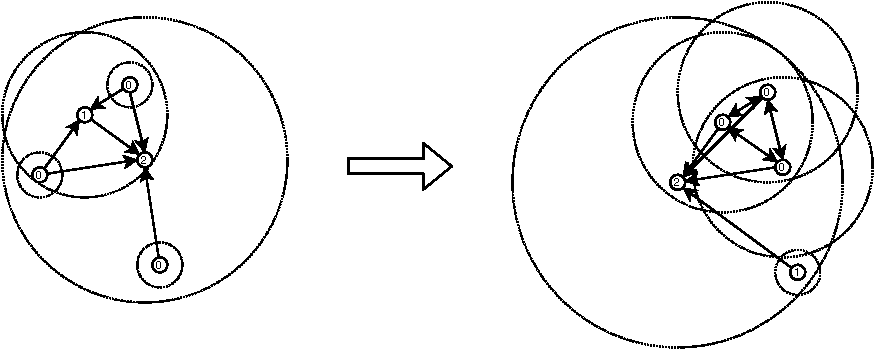
\includegraphics[width=300pt]{figures/LocarnoTreaties-Redrawing}
\caption{Redrawing the levels at each epoch can leads to very different version
    of the system. This is what is improved by the Locarno Treaties. Shrinking
    regions are depicted in red, growing regions in green and same region in
    black.} \label{fig:LocarnoTreaties-Redrawing}
\end{figure}

Following the First World War, it was decided that the borders of Germany
should remain fixed. The Locarno Treaties defined some of these borders
\cite{LocarnoTreaties TODO}. The idea of this Strawman model is to limit
modifications of regions from one epoch to the next. The idea is to use a
deterministic set of rules, based on the ping, the registrations and the map of
the previous epoch to draw the map of the current epoch using the less
redrawing as possible. CRUX is run at the first epoch giving the first version
of the system. Registration is still global and each node will have all the
information about the memberships of every node.Then from one epoch to another,
the purpose of the game is to keep as much regions as possible. The obvious
idea to reach this goal is to let the nodes conserves their levels from one
epoch to the next.  However some small difference should be introduced in order
to avoid some problems.  These are described in the next section.

\subsection{Rebalancing the levels} \label{rebalancing}
Conserving the levels is the way to go, but maintaining levels can lead to
de-equilibrated systems. Consider a system with 200 Nodes at epoch 1, with the
repartition given in Table \ref{example-lottery}. If from epoch 1 to epoch 2,
100 level-0 nodes leave the system, the remaining system would contain 80
level-0 nodes instead of 90. 

De-equilibrated systems can lead to some problems, the proof is given in the
appendix [APP. \ref{proof-reequilibrating}].

The lottery process presented in section \ref{lottery}, is a bit changed in
this part to allow the adaptation of the levels. The total number of
participants $N$ in the system is known after the registration, and as the
probability $P$ is given, it is straightforward to compute the expected number
of nodes that one should have at every level as it mentioned in Table
\ref{example-lottery}. 

Instead of drawing directly the levels from a randomness source, nodes will
draw a random number from this source between 0 and 1.  All nodes can deduce
what number the others will draw deterministically from the registration list.
The highest level will go to the node which has drawn the highest random
number.  And levels are given according to the drawing in a descending order.  

Each node that stays in the system will keep its random number from when it
joined the system, new nodes gets new random numbers. 

\subsection{Effects for a fixed node} This section describes how to transform
the regions from one epoch to another.  The point of view of one node that
stays fixed in the system is taken, the goal is that node can keep most of its
region assignment.  What are the implications. As it was said other nodes might
join, leave or move. This leads either to change in its cluster of in its
bunch. 
Additional effects can come from the level rebalancing. 

\subsubsection{Nodes Leaving the Cluster} 
This will shrink the cluster. As the regions created by a given node stops when
the radius covers the whole cluster, this might lead to the deletion of some
regions. This does not change the
region assignment and the nodes can still keep the replicated system of the
previous epoch running.

Additional effects can come from the level rebalancing. 

\subsubsection{Nodes Joining the Cluster} 
On the contrary, if nodes join the cluster, this might lead to the creation of
additional region to cover these extra nodes. The node will then replicate its
system to the newly created regions. But most of the regions are kept the same.

\subsubsection{Nodes Leaving the Bunch} 
Nodes participate to all the region in their bunch, eventually they will
participate to a region that spans the whole system. If a node left the system
in the bunch,  this leads to a region centered around a point that is not in
the system anymore, this assignment might be forgotten. 

From the point of view of a node, if another node leaves its bunch, it can have
as effect to add other nodes in its bunch, leading to more region assignment.
And in some cases, to more nodes in its cluster, leading to region growth. 

\begin{figure}[!h] 
\centering
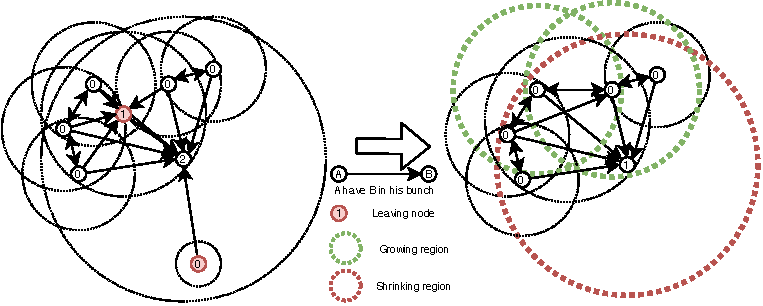
\includegraphics[width=300pt]{figures/LocarnoTreaties-Leaving-cluster}
\caption{A leaving node is changing assignments of other
    nodes but keep the same regions. Shrinking regions are depicted in red,
    growing regions in green and same region in black. }
\label{fig:LocarnoTreaties-Leaving-cluster}
\end{figure}

\subsubsection{Nodes joining the bunch} 
If nodes are joining in a bunch, this leads to additional region assignment. 

\subsection{Rules for other nodes}
Moving nodes or joining nodes are different, they are joining a new region, the
question is how to integrate them in the system while keeping the system
balanced. 

\subsubsection{Moving node example}
Assume that going from Epoch $i$ to $i+1$, one node as gone from one place to
the other end of the system. As nodes can keep their level, it will change some
of the assignments, but most of the regions will be maintained. 

\begin{figure}[!h] 
\centering
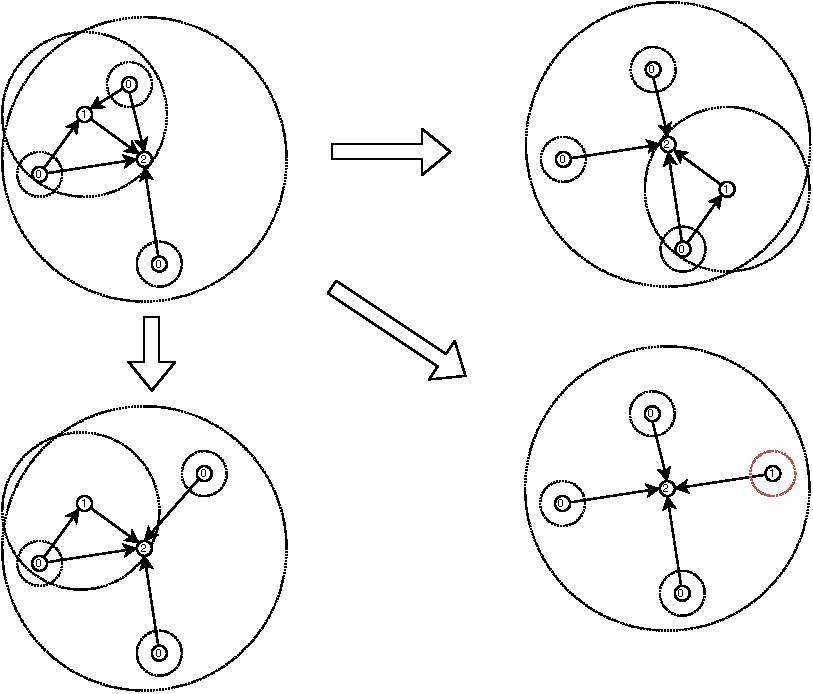
\includegraphics[width=300pt]{figures/LocarnoTreaties-Moving}
\caption{A moving node keeping its levels is changing assignments of other
    nodes but keep the same regions. Shrinking regions are depicted in red,
    growing regions in green and same region in black. }
\label{fig:LocarnoTreaties-Moving}
\end{figure}

This seems to indicate that movement should not be a problem. There is a
slight difference between that situation and redrawing the levels at each
epoch. As each node can keep its copy of the underlying system working in its
region. If the levels are redrawn, communication might be needed to transfer
knowledge from one region to another. This communication overhead is reduced in
that situation. 

\subsubsection{Leaving nodes}
Leaving nodes does not create additional problems as fixed nodes does already
know how to deal with that case. 

\subsubsection{Joining nodes}
The joining nodes can lead to the growth of one region or the creation
of regions. The precise rules for that are listed below. 

\textit{In the space-time graph (the image), most of the regions remain the same and
the modifications appear in small places.}

\begin{figure}[!h] 
\centering
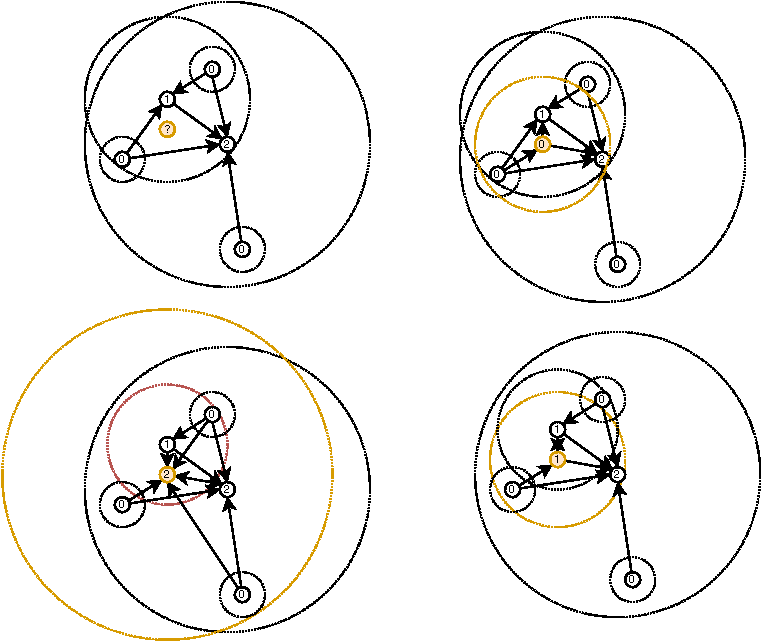
\includegraphics[width=300pt]{figures/LocarnoTreaties-Insertion-close}
\caption{Keeping the same level leads to smaller changes when a node enter the
    system. Shrinking regions are depicted in red, growing regions in green and
    same region in black.} \label{fig:LocarnoTreaties-Insertion-close}
\end{figure}

\begin{figure}[!h] 
\centering
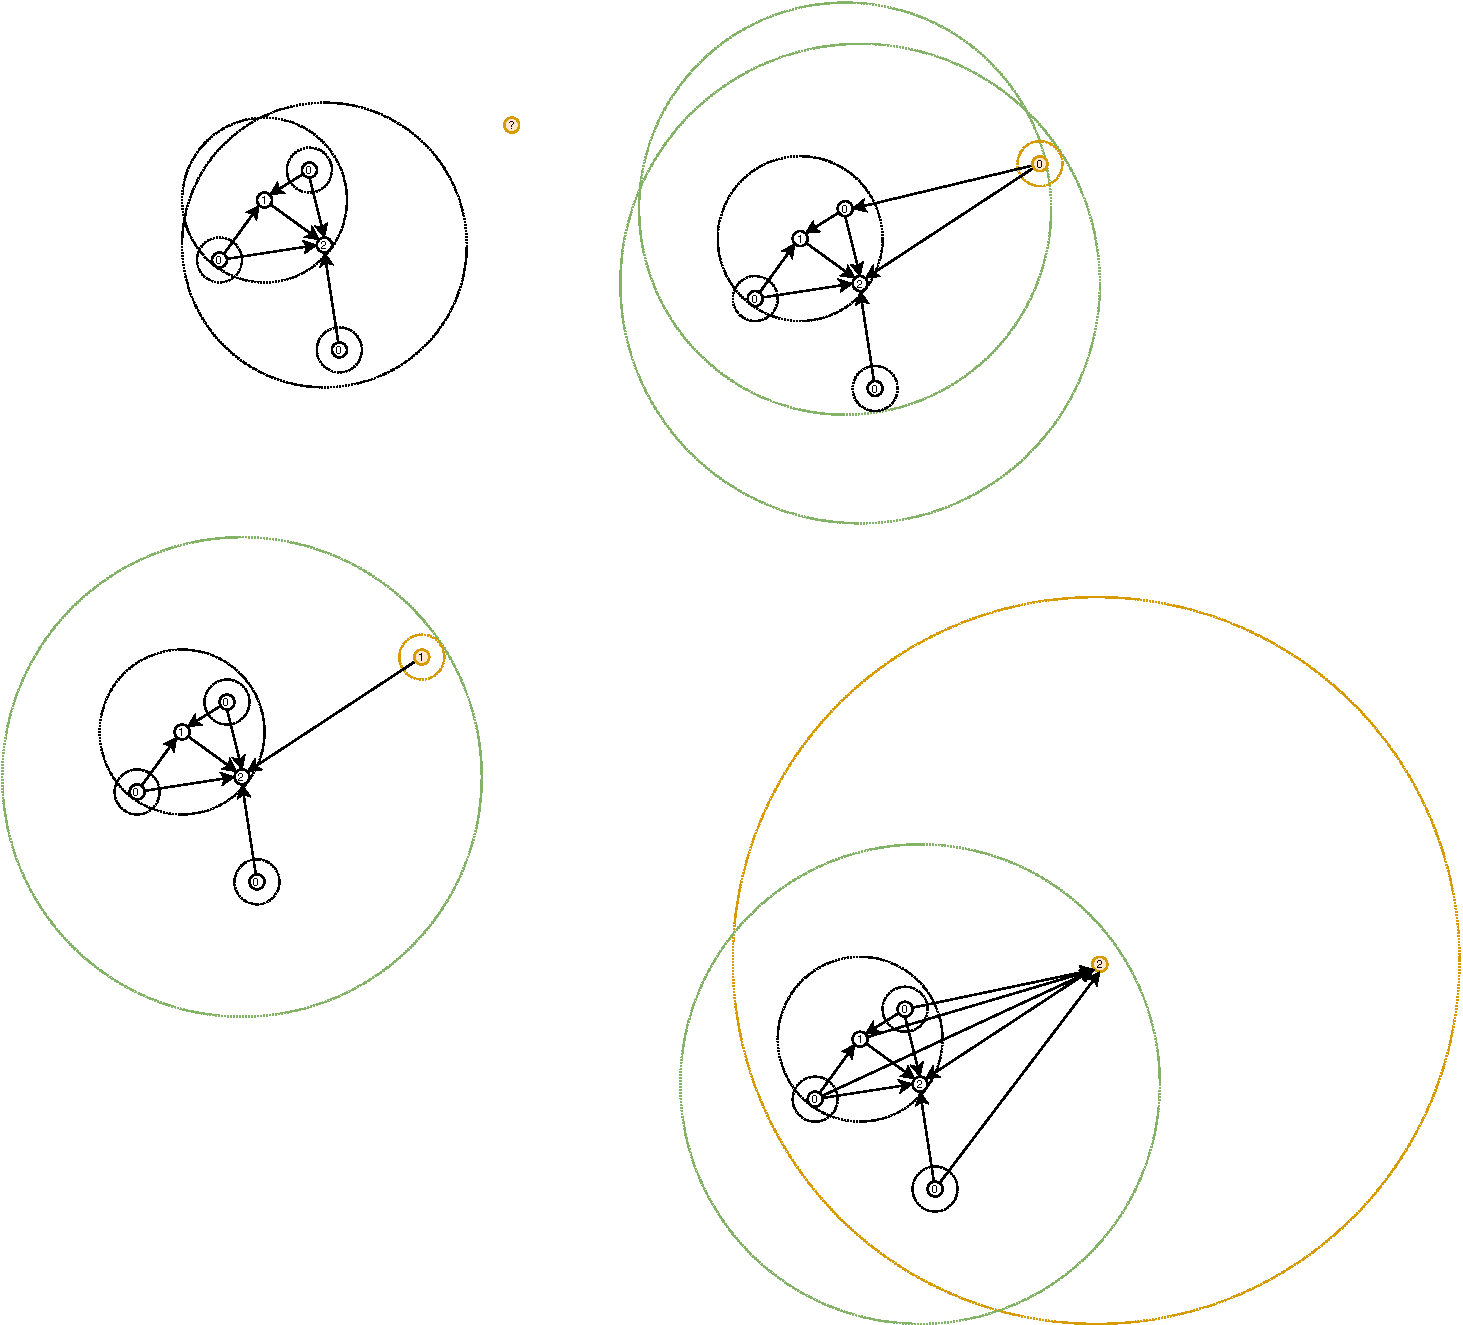
\includegraphics[width=300pt]{figures/LocarnoTreaties-Insertion-far}
\caption{Keeping the same level leads to smaller changes when a node enter the
    system. Shrinking regions are depicted in red, growing regions in green and
    same region in black.} \label{fig:LocarnoTreaties-Insertion-far}
\end{figure}

\subsection{Protocol}
The protocol is mostly the same as the simple control plane protocol [FIG.
\ref{fig:registrationprotocol}]. The main difference is the level assignment
which follows the new algorithm described in \ref{rebalancing}. 

\subsection{Threat Model}

The new lottery process can be targeted from attackers. But as it is equivalent
to the other one, attacks that are valid for one system are valid for this one.
But this will ensure to have the proper number of levels in the system in each
epoch.

If one node is not happy with its level assignment, it can leave the system a
re-enter later, hoping to get a better level. This attack works against the two
algorithms, but this attack does not create too
bad consequences, as it is presented in \ref{Threat-Model}.

Another attack could be that malicious nodes exit and re-enter the system at
each epoch until they manage to get a good number from the lottery. Then when
it manages to get good level, they collectively move to one side of the system
leaving good nodes all at level-0 in the middle of the system. This will create
a slight overhead for the good nodes as the region’s assignment increase for
the level-0 nodes. But this attack seems to cost a lot of resources and
coordination for the attacker to generate a small overhead on the size of the
participants.

Some defense mechanisms can be set up to ensure that levels are geographically
distributed over the whole system, they are described in more details in
\ref{Possible Improvements.} 

\subsubsection{Quantifying the effect of Locarno Treaties}
The goal of the new protocol is to keep most regions and region assignment
following the evolution of the system. 

A concrete comparison is made. The system starts with a fixed number of nodes
and evolves with nodes moving, leaving and entering the system. A metric is
chosen to evaluate the difference between the system from one epoch to the
next. The metric is defined as the following :  the list of participants in the
system is taken sorted by name. Then for each node, their bunch and cluster
will be compared. Each difference will be counted, if a new node enter the
system, their bunch and cluster count as a difference. Same if a node leaves
the system. The idea is that with this new protocol, the difference should be
reduced. 

The results of the experiment can be seen in [FIG. \ref{TODO FIGURE}]. Maps of
the system is given in the appendix.

\section{Strawman 2 : Fog of the War}

Each node of the system will have a different view of the world at a given time
depending on its place in the system and its interactions. Again the idea is
that one node should be aware of only the information it needs to perform its
actions. 

A correspondence can be made with the fog of war in some traditional real-time
strategy video game, where each player will have its own view of the system,
based on where it is now (real-time evolution), where it was in the past but
cannot see now (fog) and what it has not already seen (dark).

Each player view will evolve through space and time accordingly. In the context
of the game, the advantage of this view is that it hides the adversarial
strategy. In the context of our system, this view will hide most of the
information that is not relevant to one node but allow it to perform its
operation without the storage and/or communication overhead. 

The design of this Strawman will be the following. Each node declares a
position during the registration, and other nodes computes their bunch and
cluster according to this declared position. Each node will therefore be able
to compute their bunch and cluster based on these declared position. To ensure
the correctness of the system a random committee of checkers are elected after
the registration process. These checkers will perform some tests (pinging other
nodes of one region) and publish the results. 

\begin{figure}[!h] 
\centering
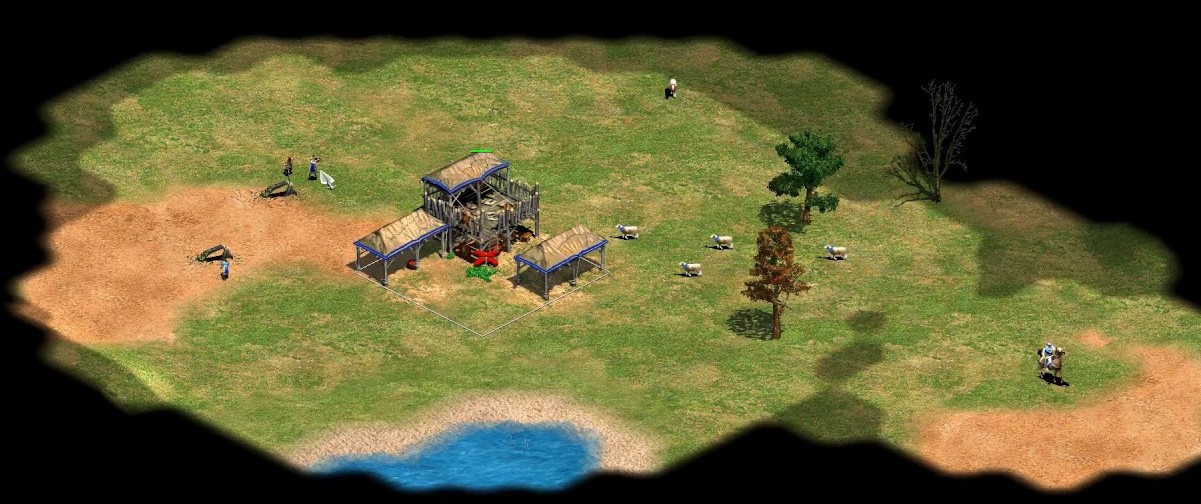
\includegraphics[width=400pt]{figures/fog_of_war}
\caption{Fog of war representation in a classic real-time strategy video game. }
\label{fig:registrationprotocol}
\end{figure}

\subsection{Purpose : Reducing the need of the Locality Component}
The protocol presented in the Simple Control Plane protocol and in the Locarno
Treaties still need a consensus on the pings between all nodes in the system.
This can be cumbersome as the number of nodes increases in the system this
quantity increases in $O(n^2)$ and consensus might become too costly. 

The idea is to change that consensus with a declared position and a random
committee of checkers. The question is still : how to choose the committee ? If
sampled randomly the chances are big that the selected nodes will be far away
from each other, and above a certain threshold, the correlation between pings
and distances are not satisfactory. Therefore the committee of checkers can be
selected to be the $N$ closest nodes based on the declared distances. And $N$
can be adapted to increase if one node does not pass the checks. 

If a node does not pass, the checks it either means that this node is faulty or
that the number of checkers is constituted of a majority of malicious nodes.
One can solve the second problem by increasing the number of checkers $N$, and
progressively a majority of honest nodes should have checked the node. It the
ping still does not correspond to what the node declared then one might assume
that the node itself is faulty. 

\begin{figure}[!h] 
\centering
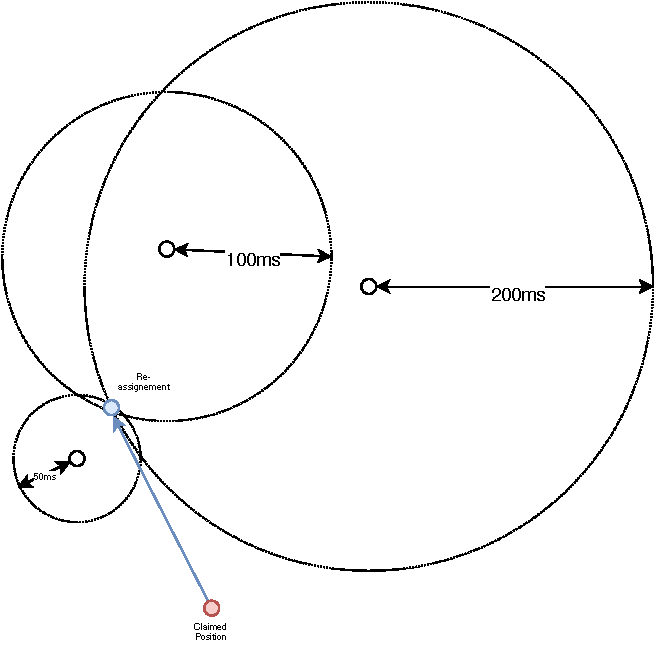
\includegraphics[width=300pt]{figures/triangulation_strategy}
\caption{Triangulation can be used to reassign the position of a faulty node.  }
\label{fig:triangulation_strategy}
\end{figure}

\subsection{Protocol}
The protocol is mostly the same as the simple control plane protocol [FIG.
\ref{fig:registrationprotocol}]. The only difference is the consensus on the
pings which are now replaced by a declared distance, which is announced before
the level assignment and a round of checks and announce of the checks. 

\subsection{Threat Model}
Another question can be, what are we supposed to do with a node that are not
passing the tests ? First it is important to notice that it won't actually
change the view that all nodes will have of the system, as nodes use the
declared distance to compute their bunch and cluster. But one node could use
that system to keep its level and go to a strategic place where it can have
more influence. This is what one may want to avoid. 

There are three approaches to this problem, the first is to exclude the node
from the system, but it might lead to the redrawing of a certain number of
regions, and it might lead to attacks. Another strategy could be to define the
position of the faulty node with an approximation based on the ping. If we have
the position of the other nodes and we have to fix the location of the unknown
faulty node one might do that by computing the intersection between the circles
based on the pings. This triangulation strategy can block one faulty node to
reach a desired position. 

As nodes can announce a position and that is checked in priority by close
nodes, with this protocol if there is a sufficient number of malicious nodes,
they can declare that they all live in a close region and valid each other.
There is no simple solution to this problem, but that fact has no consequence
on the system so it seems to be an acceptable weakness.

\section{Introducing the Space/Time metrics}

Pings give a space/time insight of the evolution of the system.  This idea can
be leveraged to create the Space/Time version of the control plane. In fact
every message (send + reply - processing time) can be transformed to be used as
a ping as well. Therefore each time a node interacts with other nodes it can
use that additional information to get insight about the evolution of the
system. 

What type of information can be inferred from this additional method ? First
nodes can track the evolution through time and space of other nodes in the
system. And react to them. For example, if a new node manages to ping an
existing node from inside one region, the already existing nodes could trigger
registration of these nodes. On the contrary, if one node starts to get away
from the rest of the region, then other nodes will notice and can decide to
kick this node out of their region (after consensus with the existing nodes).
Modifications (e.g. nodes movement, churn), can be detected directly with the
messages, and the system can react to it. Churn can be interpreted as a node
movement in this model, with the churning node moving to infinity. If one
moving node is leaving one region, this information can be propagated to the
directly upper region containing the node. 

\subsection{Information as Bubbles in Space Time Graphs}

Imagine the following situation : there is a system of some nodes divided into
regions. All nodes are fixed except one which is moving. While moving this node
is interacting with other nodes (sending messages and executing query for the
system). Other nodes detect its movement, and are capable of reacting to it.
This movement triggers some action : joining regions and leaving others. If the
node is moving slowly, the reaction stays local, as information only needs to
be propagated in some upper region to be resolved. On the contrary, if the node
moves fast, then it generates bigger bubbles, it goes to the biggest region to
be resolved.  Structurally this view of the system is not really different from
the one that we described before, but philosophically this view goes much
deeper as it taking in account the interactions of the nodes in a space/time
matter.

In terms of Nyle components, the locality component has an additional view and
can influence first the region component. Registration is still global, epochs
managed the rhythm for the registration. Instead of only having a locality
measure at the beginning of the epoch, this view allows to have measures of the
system dynamically at all time. 

This can be used to adapt the region assignment during the system. At first the
regions will be kept the same with fixed borders but the rules for region
assignment can be stated. 

\subsubsection{Rules for Region Assignment based on the Space/Time Metric}
Recall that nodes participate to all region that is bigger than its cluster. If
nodes in one region detect that another is moving apart, they do not expect it
to participate in this region anymore and they propagate the information in the
directly upper region. This is done recursively till the node is again included
in the more global region.  In the opposite, if a region detect that one node
is approaching it expects it to participate in the region, and propagate the
information in the directly upper region.

If a node churns, then this information is propagated all the way to the
biggest region, and the node is excluded from all the regions. 

\subsubsection{Transformation of regions}
This change in region assignment actually have an effect on the form of the
region, the same rules developed in \ref{Locarno} can be applied to adapt the
regions on the fly. 

\paragraph{Protocol}
If node $A$ is moving and leaves a region, and another node $B$ detects that
while communicating with $A$, it will take that in account meaning it will
store the last ping and adopt its own view on the system. If a major change is
detected, for example that $A$ leaves the cluster of $B$ leading to the
shrinking of the cluster of $B$ then $B$ will notify the other nodes
participating in its cluster that it shrank the region. It will as well notify
the first node of its bunch, and provide the ping. This will start a recursive
reaction, nodes in the directly bigger region will start pinging $A$, if it is
still in the region it can be integrated in another region. If $A$ moved too
fast, it might have left its cluster as well, so the information would be
transferred to the next bigger region. Eventually the biggest region, which
covers the whole system would be reached. 

\subsubsection{Rules for Membership Component based on the Space/Time metric}
The Space/Time Metric can be leveraged to serve as a Membership Components.
Decisions are made on the majority of nodes. To be able to participate in
the system or to take part in a decision, a valid endorsement in required. If a
node churns, then this information is propagated all the way to the
biggest region, and the node is excluded from the system.  If a node joins the
system, it starts to ping some nodes for information. It can ask for the list
of participants and pings everybody. When it starts pinging some nodes that are
close to it, these nodes detect that a new node wants to join the system and
when nodes are aware of the place of the new participant, it can be verified by
a random number of checkers. The verification will check that the place is
actually right and that a valid \textit{endorsement} is provided, and a level
will be given to it. 

\subsubsection{Epoch Components}
With the Membership adaptation and the transformation of the regions, there is
no need for epochs anymore. This component can be deleted from the system. 

\subsection{Space/Time Protocol}
Assume that we have a precisely defined set of rules for evolving the region
from one epoch to another.  The Space/Time Protocol will be the following.
Regions are created in the genesis of the system by the algorithm for region
creation. The underlying system is replicated in all the deployed regions. And
nodes start working in the system. Events are detected with the dynamic
Space/Time Metric. 

\subsection{Threat model}
Malicious nodes might forge ping to let other nodes thinking that a good node have moved. 

%% TODO CONTINUE 

%%%%%%%%%%%%%%%%%%%%
\chapter{Possible Improvements}
%%%%%%%%%%%%%%%%%%%%

This chapter lists the improvements that could be applied more or less directly
to one part of the project, but that were not implemented due to time reasons. 

In the simple control plane protocol, the live clock that are supposed to be
synchrone for every nodes could be replaced by Timestamps Logical Clocks (TLC)
\cite{Que-Sera-Consensus}. This could allow the system to be more flexible.
This replace the clock and succeed the registration and the live period.
However, this was not implemented as it was hard to see how to go from one
epoch to another using TLC. Recall that in the existing protocol, at the
beginning of the live period one node of the old committee sends the necessary
information to the new committee to begin. Synchronizing this could be hard.

%%%%%%%%%%%%%%%%%%%%
\chapter{Conclusion}
%%%%%%%%%%%%%%%%%%%%

In the conclusion you repeat the main result and finalize the discussion of
your project. Mention the core results and why as well as how your system
advances the status quo.

\cleardoublepage \phantomsection \addcontentsline{toc}{chapter}{Bibliography}
\printbibliography

% Appendices are optional \appendix %%%%%%%%%%%%%%%%%%%%%%%%%%%%%%%%%%%%%%
% \chapter{How to make a transmogrifier} %%%%%%%%%%%%%%%%%%%%%%%%%%%%%%%%%%%%%%
%
% In case you ever need an (optional) appendix.
%
% You need the following items: \begin{itemize} \item A box \item Crayons \item
% A self-aware 5-year old \end{itemize}

\end{document}
